\section{Profiling Motivation}
Haskell provides a mechanism to allow the user to control the granularity of parallelism by indicating what computations may be usefully carried out in parallel. This is done by using functions from the \codef{Control.Parallel} module. The interface for \codef{Control.Parallel} is shown below:
\begin{lstlisting}[columns=flexible]
  par  :: a -> b -> b 
  pseq :: a -> b -> b 
\end{lstlisting}
The function \codef{par} indicates to the GHC run-time system that it may be beneficial to evaluate the first argument in parallel with the second argument. The \codef{par} function returns as its result the value of the second argument. One can always eliminate \codef{par} from a program by using the following identity without altering the semantics of the program:
\begin{lstlisting}
  par a b = b 
\end{lstlisting}
A thread is not necessarily created to compute the value of the expression \codef{a}. Instead, the GHC run-time system creates a {\em spark} which has the potential to be executed on a different thread from the parent thread. A sparked computation expresses the possibility of performing some speculative evaluation. Since a thread is not necessarily created to compute the value of \codef{a}, this approach has some similarities with the notion of a {\em lazy future}~\cite{mohr:91}.

% SDM: removed, not necessary for the Haskell Symposium.  Also the
% following paragraph doesn't make sense.
%
% Sometimes it is convenient to write a function with two arguments as an
% infix function and this is done in Haskell by writing backticks 
% around the function:
% \begin{lstlisting}
%   a `par` b
% \end{lstlisting}

We call such programs semi-explicitly parallel because the programmer has provided a hint about the appropriate level of granularity for parallel operations and the system implicitly creates threads to implement the concurrency. The user does not need to explicitly create any threads or write any code for inter-thread communication or synchronization.

To illustrate the use of \codef{par} we present a program that performs two compute intensive functions in parallel. The first compute intensive function we use is the notorious Fibonacci function:
\begin{lstlisting}
fib :: Int -> Int
fib 0 = 0
fib 1 = 1
fib n = fib (n-1) + fib (n-2)
\end{lstlisting}
The second compute intensive function we use is the \codef{sumEuler} function taken from~\cite{trinder:02}:
\begin{lstlisting}
mkList :: Int -> [Int]
mkList n = [1..n-1]

relprime :: Int -> Int -> Bool
relprime x y = gcd x y == 1

euler :: Int -> Int
euler n = length (filter (relprime n) (mkList n))

sumEuler :: Int -> Int
sumEuler = sum . (map euler) . mkList
\end{lstlisting}
The function that we wish to parallelize adds the results of calling \codef{fib} and \codef{sumEuler}:
\begin{lstlisting}
sumFibEuler :: Int -> Int -> Int
sumFibEuler a b = fib a + sumEuler b
\end{lstlisting}
As a first attempt we can try to use \codef{par} to speculatively spark off the computation of \codef{fib} while the parent thread works on \codef{sumEuler}:
\begin{lstlisting}
-- A wrong way to parallelize f + e
parSumFibEuler :: Int -> Int -> Int
parSumFibEuler a b
  = f `par` (f + e)
    where
    f = fib a
    e = sumEuler b
\end{lstlisting}

To create two workloads that take roughly the same amount of time to
execute we performed some experiments which show that \codef{fib 38}
takes roughly the same time to execute as \codef{sumEuler 5300}.  The
execution trace for this program as displayed by ThreadScope is shown
in Figure~\ref{f:wrongpar}. This figure shows the execution trace of
two Haskell Execution Contexts (HECs), where each HEC corresponds to a
processor core.  The $x$-axis is time.  The purple portion of each
line shows at what time intervals a thread is running and the orange
(lighter coloured) bar shows when garbage collection is occurring.
Garbage collections are always ``stop the world'', in that all Haskell
threads must stop during GC, but a GC may be performed either
sequentially on one HEC or in parallel on multiple HECs; in
Figure~\ref{f:wrongpar} we are using parallel GC.

\begin{figure*}
\begin{center}
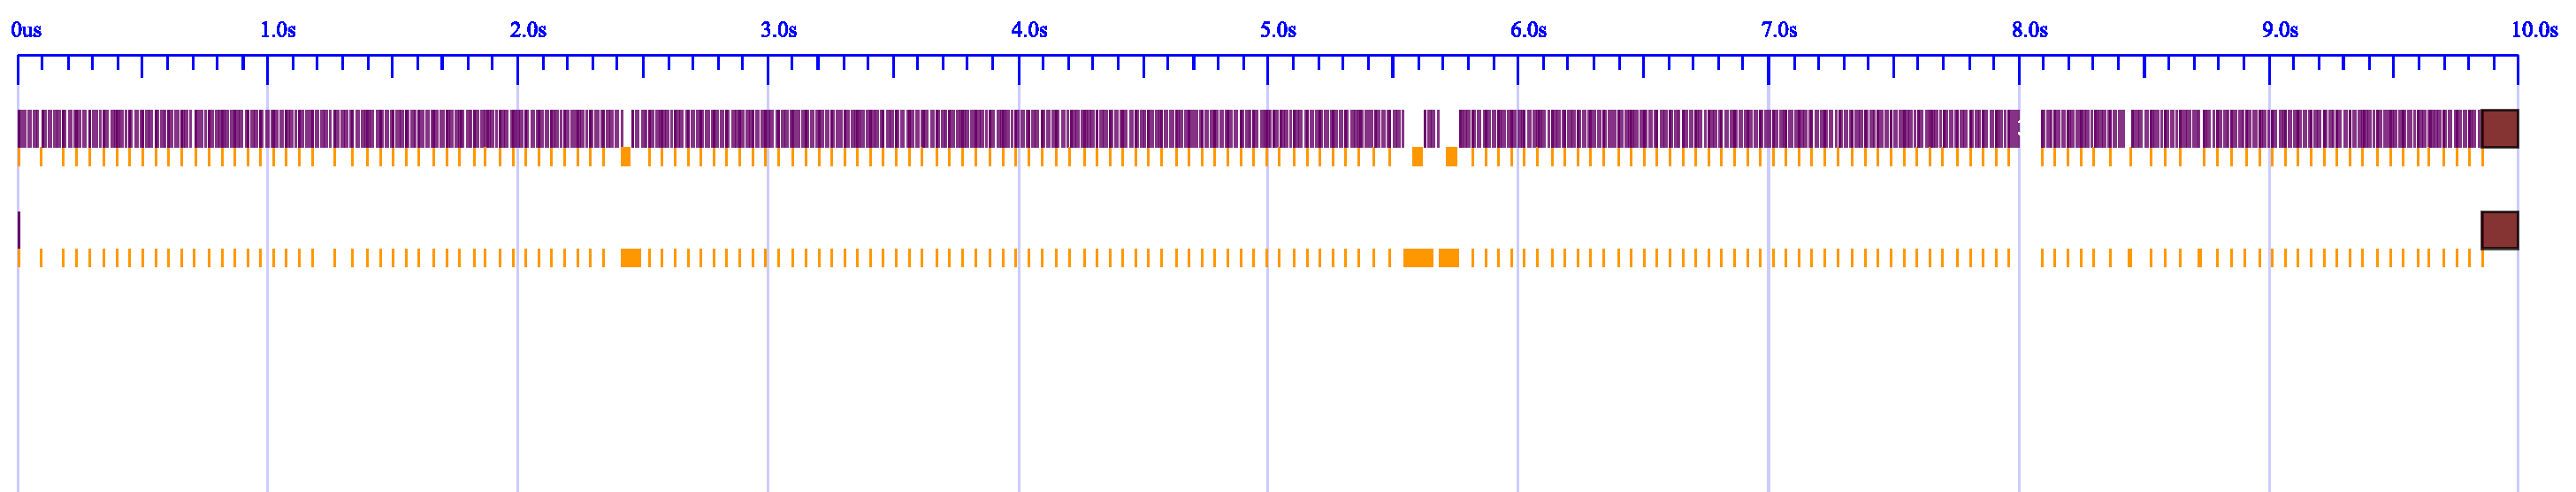
\includegraphics[width=18cm]{SumEuler1-N2-eventlog.pdf}
\end{center}
\caption{No parallelization of \codef{f `par` (f + e)}}
\label{f:wrongpar}
\end{figure*}

We can examine the statistics produced by the runtime system (using
the flags \texttt{+RTS -s -RTS}) to help understand what went wrong:

\begin{verbatim}
  SPARKS: 1 (0 converted, 0 pruned)

  INIT  time    0.00s  (  0.00s elapsed)
  MUT   time    9.39s  (  9.61s elapsed)
  GC    time    0.37s  (  0.24s elapsed)
  EXIT  time    0.00s  (  0.00s elapsed)
  Total time    9.77s  (  9.85s elapsed)
\end{verbatim}

The log shows that although a single spark was created, no sparks
where ``converted'', i.e. executed.  In this case the performance bug
is because the main thread immediately starts to work on
the evaluation of \codef{fib 38} itself which causes this spark to
\emph{fizzle}.  A fizzled spark is one that is found to be under
evaluation or already evaluated, so there is no profit in evaluating
it in parallel. The log also shows that the total amount of
computation work done is 9.39 seconds (the \codef{MUT} time); the time
spent performing garbage collection was 0.37 seconds (the \codef{GC}
time); and the total amount of work done amounts to 9.77 seconds with
9.85 seconds of wall clock time. A profitably parallel program will
have a wall clock time (elapsed time) which is less than the total
time\footnote{although to measure actual parallel speedup, the wall-clock time
  for the parallel execution should be compared to the wall-clock time
  for the sequential execution.}.

One might be tempted to fix this problem by swapping the arguments to
the \codef{+} operator in the hope that the main thread will work on
\codef{sumEuler} while the sparked thread works on \codef{fib}:

\begin{lstlisting}
-- Maybe a lucky parallelization
parSumFibEuler :: Int -> Int -> Int
parSumFibEuler a b
  = f `par` (e + f)
    where
    f = fib a
    e = sumEuler b
\end{lstlisting}

This results in the execution trace shown in Figure~\ref{f:lucky} which shows a sparked thread being taken up by a spare worker thread. 

\begin{figure*}
\begin{center}
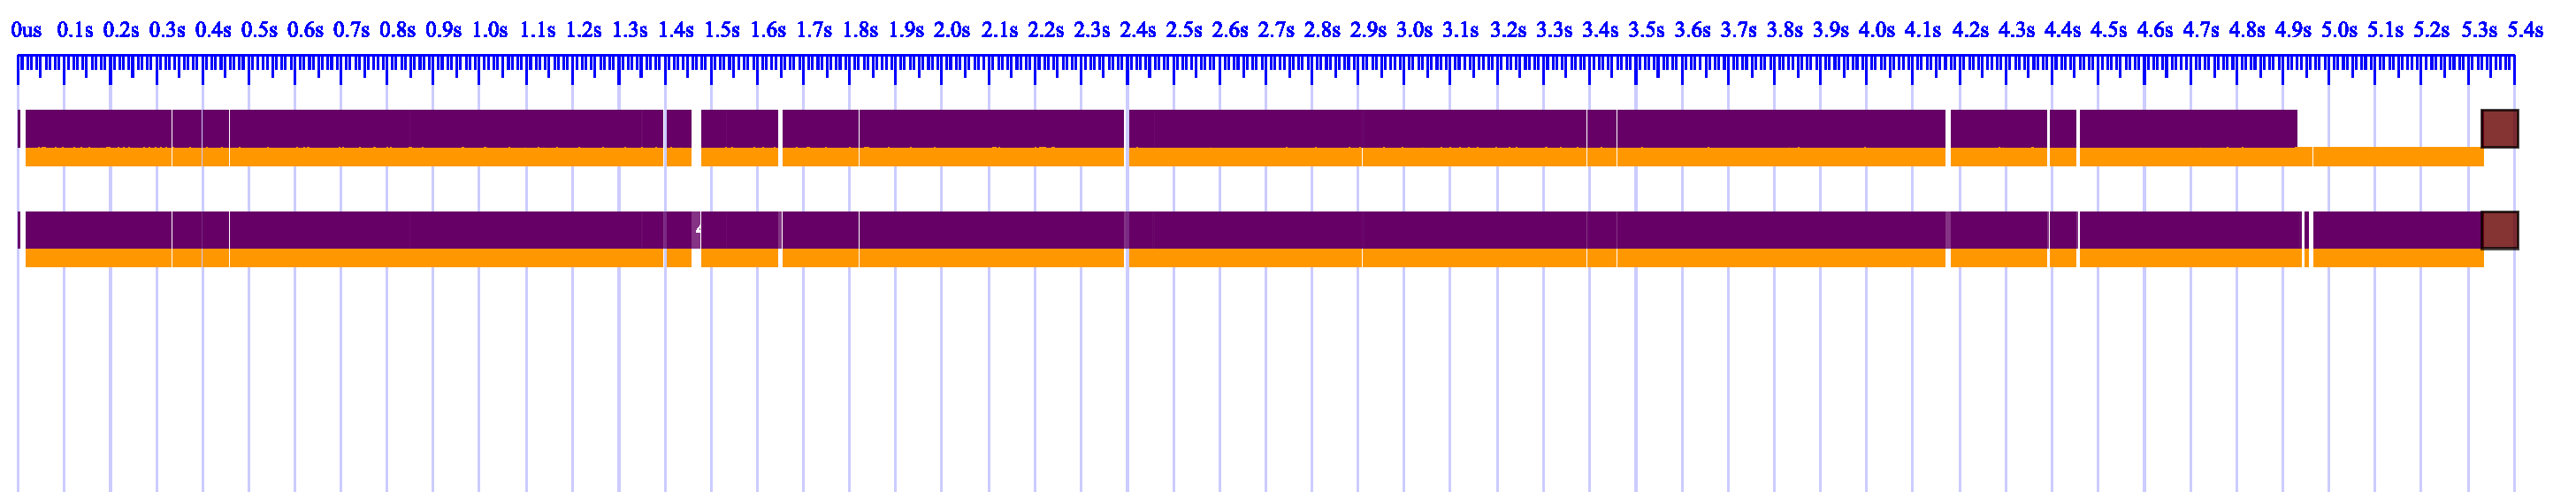
\includegraphics[width=18cm]{SumEuler2-N2-eventlog.pdf}
\end{center}
\caption{A lucky parallelization of \codef{f `par` (e + f)}}
\label{f:lucky}
\end{figure*}

The execution log for this program shows that a spark was used productively and the elapsed time has dropped from 9.85s to 5.33s:

\begin{verbatim}
  SPARKS: 1 (1 converted, 0 pruned)

  INIT  time    0.00s  (  0.00s elapsed)
  MUT   time    9.47s  (  4.91s elapsed)
  GC    time    0.69s  (  0.42s elapsed)
  EXIT  time    0.00s  (  0.00s elapsed)
  Total time   10.16s  (  5.33s elapsed)
\end{verbatim}

While this trick works, it only works by accident.  There is no fixed
evaluation order for the arguments to \codef{+}, and GHC might decide
to use a different evaluation order tomorrow.  To make the parallelism
more robust, we need to be explicit about the evaluation order we
intend.  The way to do this is to use \codef{pseq}\footnote{Previous
  work has used \codef{seq} for sequential evaluation ordering, but
  there is a subtle difference between Haskell's \codef{seq} and the
  operator we need for sequencing here.  The details are described in
  \citet{multicore-ghc}.} in combination with
\codef{par}, the idea being to ensure that the main thread works on
\codef{sumEuler} while the sparked thread works on \codef{fib}:

\begin{lstlisting}
-- A correct parallelization that does not depend on
-- the evaluation order of +
parSumFibEuler :: Int -> Int -> Int
parSumFibEuler a b
  = f `par` (e `pseq` (f + e))
    where
    f = fib a
    e = sumEuler b
\end{lstlisting}

This version does not make any assumptions about the evaluation order
of \codef{+}, but relies only on the evaluation order of \codef{pseq},
which is guaranteed to be stable.

This example as well as our wider experience of attempting to write semi-explicit parallel programs shows that it is often very difficult to understand if and when opportunities for parallelism expressed through \codef{par} are effectively taken up and to also understand how operations like garbage collection influence the performance of the program. Until recently one only had available high level summary information about the overall execution of a parallel Haskell program. In this paper we describe recent improvements to the Haskell run-time which allow a much more detailed profile to be generated which can then be used to help debug performance problems.
